\documentclass[conference]{IEEEtran}
\usepackage[T1]{fontenc}
\usepackage[utf8]{inputenc}
\usepackage{graphicx}
\usepackage{booktabs}
\usepackage{amsmath,amssymb}
\usepackage{algorithm}
\usepackage{algorithmic}
\usepackage{textcomp}
\usepackage{multirow}
\graphicspath{{paper_assets/diagrams/}{paper_assets/figures/}}

\begin{document}

\title{EcoMind AI: An Adaptive Explainable Energy Intelligence Platform for Data Quality-Aware Decision Support}

\author{\IEEEauthorblockN{Bindhushree B M, Kushal Gowda G, Mohith Gowda H, and Shashank Gowda N C}
\IEEEauthorblockA{Corresponding author: shashankgowdanc@gmail.com}}

\maketitle

\begin{abstract}
Forecasting energy demand from building meter data is rarely limited by the model. In practice the datasets that reach the training step are incomplete, irregular, and full of sensor artifacts, and most pipelines never check them before fitting a regressor. Worse, the pipeline itself can quietly leak the target through feature engineering performed before the train--test split. We present EcoMind AI, an offline platform in which data quality assessment, preprocessing, feature engineering, prediction, benchmarking, explanation, and confidence evaluation operate as one explicit, auditable workflow. The platform first runs a dedicated data quality engine that scores eight rules under five dimensions, then transforms and derives features, benchmarks regressors on a chronological holdout, explains every model with SHAP, compares raw versus cleaned inputs, and finally fuses four evidence factors into a single trust score before any recommendation is shown. On an hourly electricity dataset of 3,600 rows across five assets, all quality rules pass with per-rule scores between 96.7 and 100, gradient boosting leads the legitimate models with $R^2 = 0.9175$, and the trust gate reports 94.5/100 (high trust). We also record an honest null result: cleaning changed nothing here because the input was already clean, and we document a target-leakage artifact that drove ridge regression to a perfect but meaningless score.
\end{abstract}

\begin{IEEEkeywords}
data quality, energy forecasting, explainable AI, SHAP, trust, MLOps
\end{IEEEkeywords}

\section{Introduction}

Building energy datasets are not ready to be modeled the moment they are exported. Meter files arrive with null cells, duplicate timestamps, stuck sensors that report constant values, and occupants or equipment that produce values outside any physical range. We built EcoMind AI after noticing that most pipelines in this space solve the modeling part well and treat everything before it as plumbing. That assumption caused real trouble during our own experiments: a clean-looking file could still fail on timestamp continuity, and a feature we derived before validation made a linear model look perfect while the numbers meant nothing.

Our view is that prediction quality is downstream of data quality, and that trust in a forecast is downstream of being able to show \emph{why} a number is trustworthy. So the platform is organized as an explicit sequence of seventeen stages, from ingestion to a final registry, and every stage is persisted and streamed to the browser. Nothing runs on the cloud; the dataset files never leave the host machine.

The contribution of this paper is not a new learning algorithm. It is an integrated workflow in which quality assessment, preprocessing, explainable AI, raw-versus-processed comparison, confidence evaluation, anomaly detection, benchmarking, and executive decision support operate together inside one transparent pipeline. We report implementation details and measured results from the running system, including the failure modes it caught.

\section{Related Work}

Most published systems end where EcoMind AI begins. Data-driven building energy studies typically select a regressor and report accuracy on a fixed split~\cite{amasyali:2018, chen:2016}; large public corpora such as BDG2~\cite{miller:2020} are used almost exclusively as a benchmark playground rather than as a quality audit. Generic machine learning frameworks provide the regressors we reuse~\cite{breiman:2001, pedregosa:2011}, and the temporal-validation and leakage literature~\cite{bergmeir:2012, hyndman:2021} motivated our chronological holdout. The idea that data quality has many independent dimensions is not new~\cite{wang:1996}; what is missing is a runtime that enforces it inside the modeling loop instead of leaving it to a report.

Four differences position the platform. Existing systems predict; EcoMind AI validates the data first. Existing systems detect anomalies; EcoMind AI also measures how much the model can be trusted. Existing systems stop after delivering a forecast; EcoMind AI ends in an executive summary and a registry so the entire run can be audited later. Finally, where other tools suppress failed artifacts, we chose to surface ours: the paper reports a leakage case and a null result as first-class outcomes.

\begin{table}[!t]
\caption{Compared against representative families of related tools}
\label{tab:compare}
\centering
\begin{tabular}{@{}p{0.16\textwidth}p{0.22\textwidth}p{0.22\textwidth}p{0.22\textwidth}@{}}
\toprule
Capability & Prediction studies~\cite{amasyali:2018,chen:2016} & Generic ML frameworks~\cite{pedregosa:2011} & EcoMind AI \\
\midrule
Data quality scoring & no & no & separate engine, 8 rules \\
Retrospective leakage check & no & no & explicit \\
Chronicle holdout & common & optional & enforced \\
Explainability & rare & partial & built-in SHAP \\
Trust verdict & no & no & 4-factor gate \\
Raw-vs-processed & no & no & run-level \\
Executive report & no & no & generated \\
\bottomrule
\end{tabular}
\end{table}

\section{System Overview}

\begin{figure*}[!t]
\centering
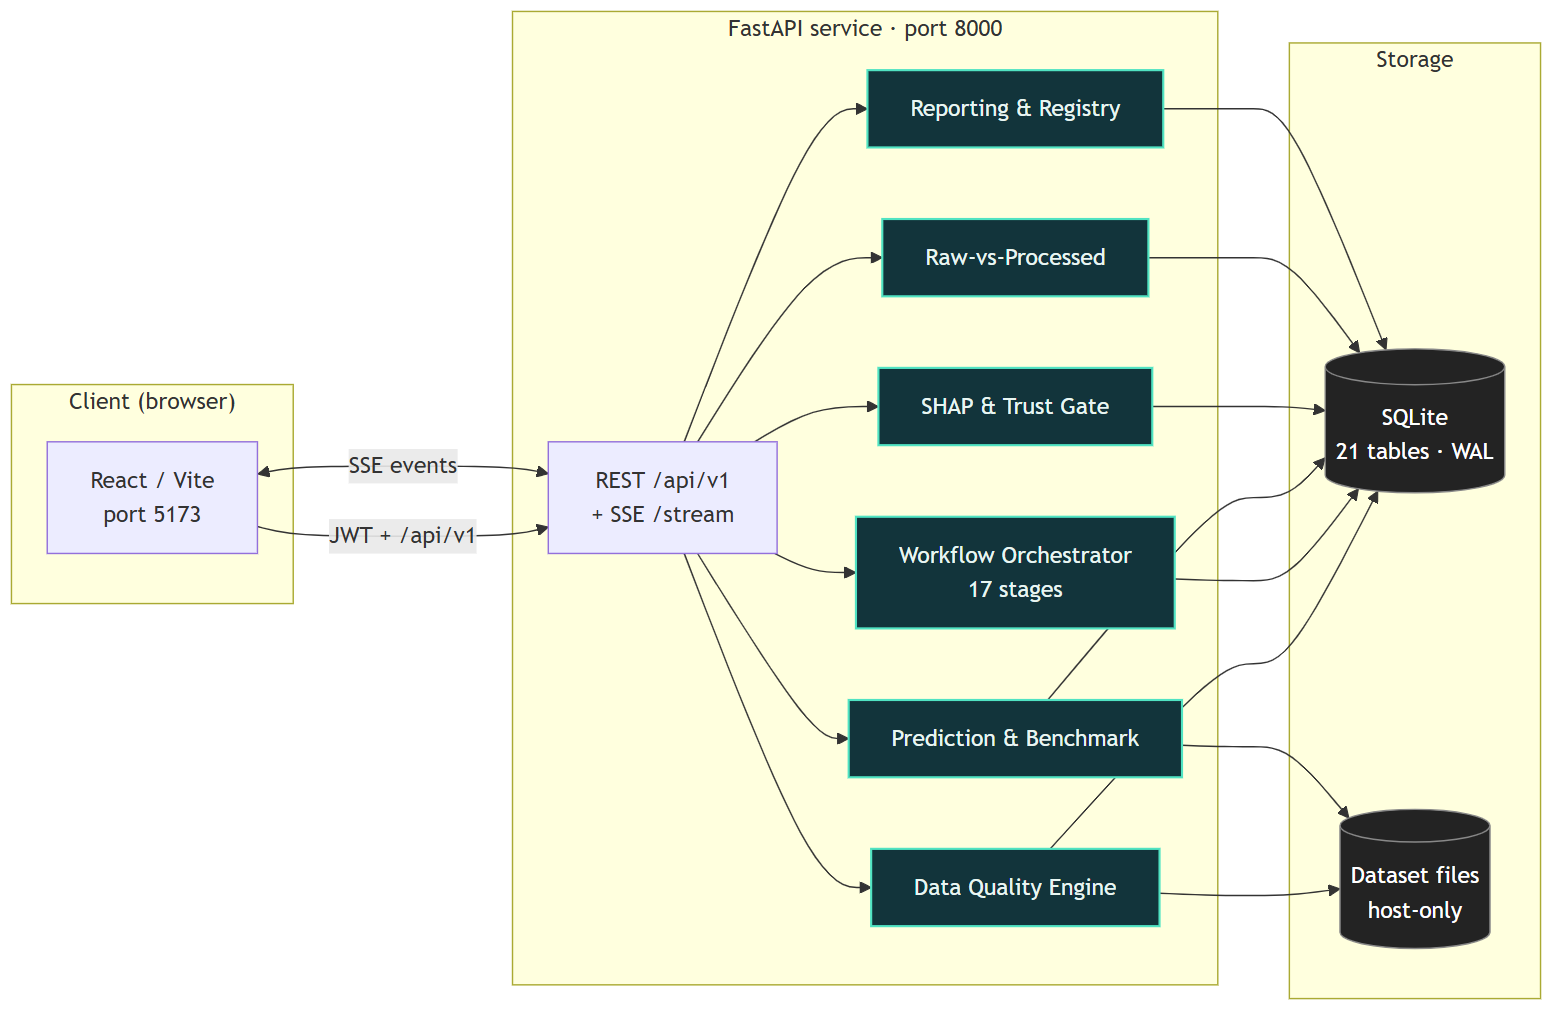
\includegraphics[width=\textwidth]{paper_assets/diagrams/system-architecture.png}
\caption{The three tiers of EcoMind AI. The React client calls a FastAPI service over a JWT-authenticated REST surface and an SSE channel for live workflow events. Domain services cover data quality, orchestration, prediction and benchmarking, SHAP explanation, raw-versus-processed comparison, the trust gate, reporting, and a model registry, all persisting to a single SQLite file.}
\label{fig:arch}
\end{figure*}

The system (Fig.~\ref{fig:arch}) runs as a React client on port 5173 that proxies requests to a FastAPI backend on port 8000. All 55 endpoints sit under \texttt{/api/v1}; authentication is a JWT issued from a default local account. State lives in one SQLite database with 21 tables in WAL mode, which keeps the whole deployment copyable to a laptop and means a run can be inspected weeks later from the history screen alone. The workflow stages are coordinated by a service that exposes \texttt{/start}, per-stage \texttt{exec}, and an SSE stream so the browser shows progress as it happens. During development we found this explicit event stream to be the single most useful debugging facility: a stuck stage was visible immediately instead of surfacing as a mysterious timeout.

\subsection{Data Model and Registry}

Persistence is deliberately boring. Twenty-one tables in SQLite hold users, datasets, workflow runs, per-rule quality results, transformations, models, benchmarks, raw-versus-processed comparisons, anomalies, recommendations, and reports. Each run pins its dataset hash and feature set, so results stay reproducible across sessions. The registry table maps the promoted model to its training rows, feature count, and dataset, and because everything is local we can query history directly with plain SQL---an ability we used constantly while diagnosing the leakage artifact of Section~\ref{sec:feat}.

\section{Methodology}

The workflow below is the heart of the platform. Each stage exists because something in a prior attempt produced a confusing result without it.

\subsection{Dataset Library and Schema Discovery}

The library lists uploaded datasets with size, row count, and column statistics. Schema discovery is deliberately separate from quality assessment: it reports types, non-null counts, and uniqueness per column, which tells the operator what can be modeled before we decide whether it can be trusted. We observed early on that assuming every ``timestamp'' column was parseable produced silent failures, so the stage re-parses and re-checks the timestamp column explicitly rather than trusting the import.

\subsection{Data Quality Engine}

The data quality engine is the signature stage, and it exists because cleaning without measurement is guesswork. During an early evaluation we dropped rows, filled gaps, and saw accuracy \emph{fall} on some datasets. That is why the engine scores every rule on a 0--100 scale, stores the details, and treats a failing rule as a control-flow event rather than a warning. The eight rules map onto Wang and Strong's dimensions~\cite{wang:1996}: completeness (null cells), two validity rules (semantic bounds and identifier blanks), two consistency rules (duplicates and timestamp monotonicity), two accuracy rules ($3\times$IQR fences~\cite{tukey:1977} and $|z|>5$ on the target), and one timeliness rule (gaps beyond $1.5\times$ the median interval). A result passes when the score is at least 80 for informational rules and 70 for critical ones.

\begin{figure}[!t]
\centering
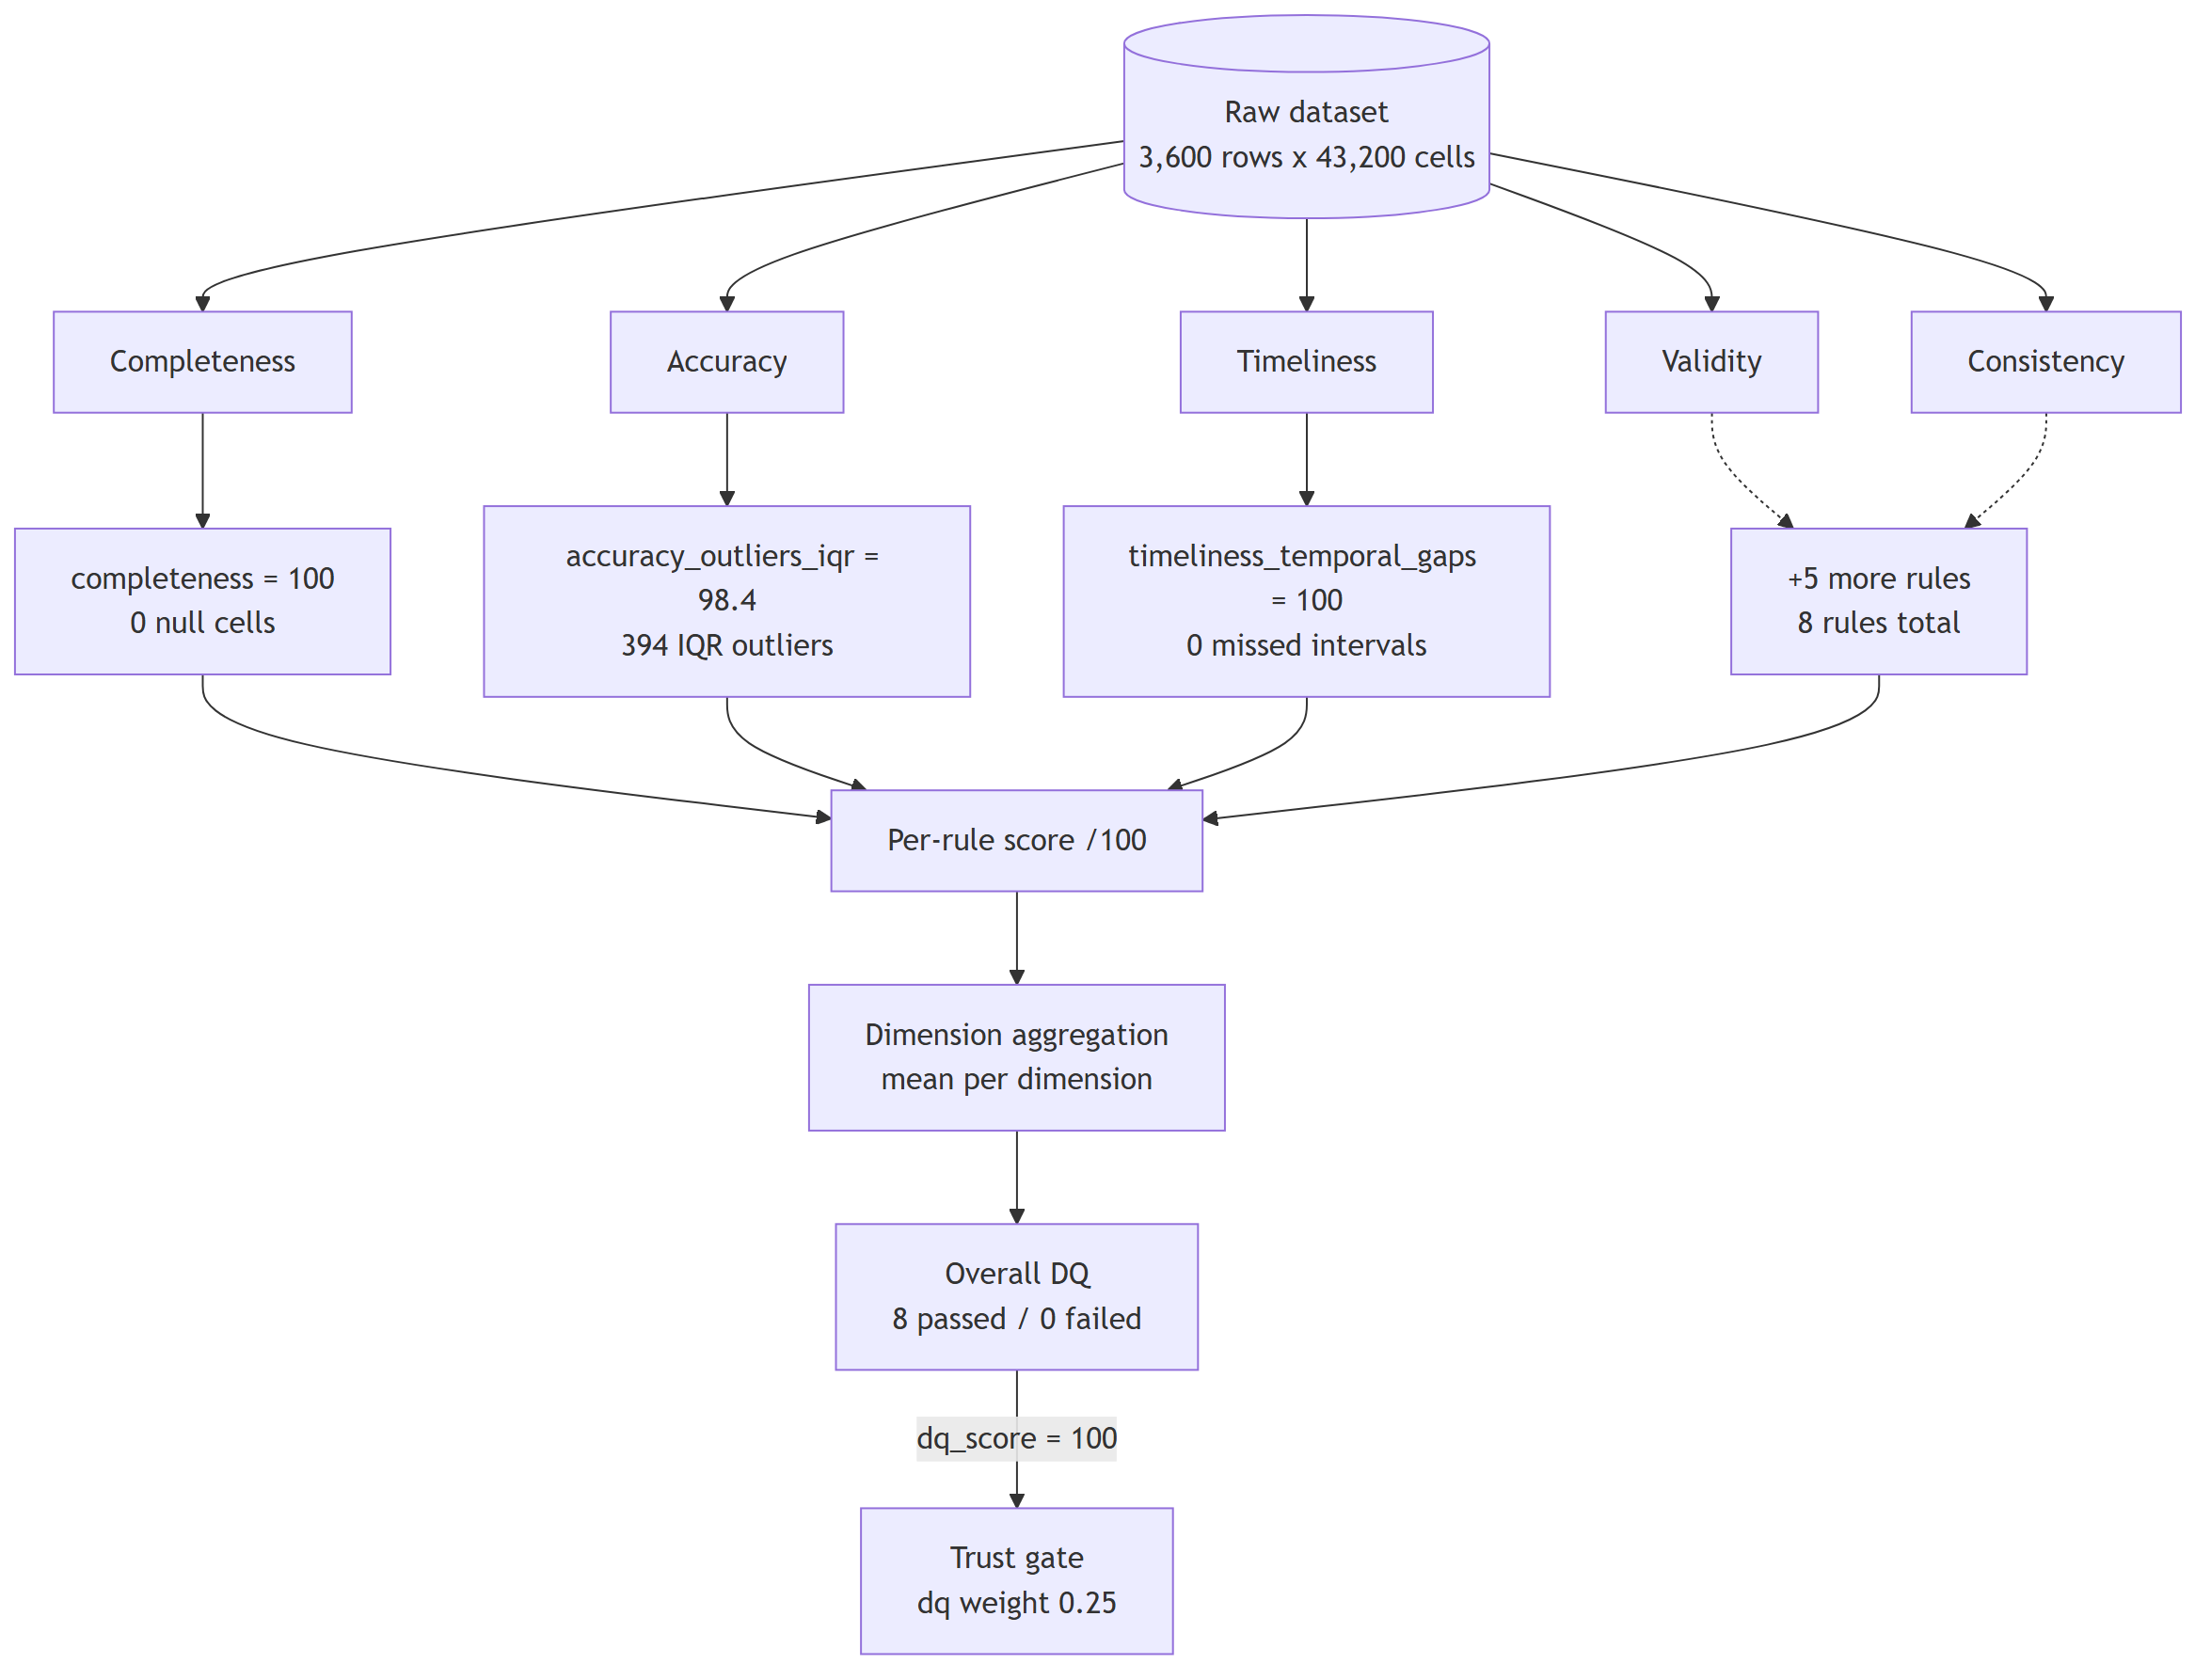
\includegraphics[width=\columnwidth]{paper_assets/diagrams/data-quality-flow.png}
\caption{The eight data quality rules grouped into five dimensions, with the score clamped and the pass/fail threshold applied per rule. Rule details are persisted so a failure can be traced later.}
\label{fig:dq}
\end{figure}

Two details from implementation are worth recording. First, the outlier rule clamps \texttt{100*(1 - min(rate, 0.5))} to the range $[50,100]$, so a pathological column can never engineer a misleadingly high ``pass.'' Second, the timestamps are not assumed hourly: the interval median is measured from the data itself, which is what makes the rule work on daily datasets without reconfiguration.

We also hit a genuine bug here that we want to document rather than hide. The aggregate score returned by the read endpoint is computed as the sum of all rule scores divided by the number of distinct dimensions ($795/5 = 159$ for the profile below), while the write path weights five dimension means by 0.25 each, capping the maximum at 125. Neither number is a percentage. Rather than ship a misleading ``/100,'' the UI reports per-rule scores and the trust gate consumes the normalized quality factor. The aggregation defect is logged for correction.

\begin{table}[!t]
\caption{Data quality profile on the reference dataset (0--100 per rule)}
\label{tab:dq}
\centering
\begin{tabular}{@{}llr@{}}
\toprule
Rule & Dimension & Score \\
\midrule
completeness & completeness & 100 \\
validity\_semantic\_bounds & validity & 100 \\
consistency\_duplicates & consistency & 100 \\
consistency\_monotonic & consistency & 96.7 \\
validity\_identifiers & validity & 100 \\
accuracy\_outliers\_iqr & accuracy & 98.4 \\
accuracy\_zscore & accuracy & 99.9 \\
timeliness\_temporal\_gaps & timeliness & 100 \\
\midrule
passed / failed & --- & 8 / 0 \\
\bottomrule
\end{tabular}
\end{table}

On the reference dataset (3,600 rows $\times$ 12 columns, 43,200 cells, five assets sampled hourly for 30 days, target \texttt{energy\_kwh}), all eight rules pass (Table~\ref{tab:dq}). Completeness is exact, all 18,000 semantic-bound checks hold, and there are no duplicates. The two imperfect scores were genuinely informative: 120 non-monotonic timestamps (96.7) and 394 IQR outliers concentrated in occupancy, energy, and power (98.4). Without the engine, none of that would have been visible before training.

\subsection{Transformation and Feature Engineering}\label{sec:feat}

The transformation viewer shows exactly which operations replay on the data, because preprocessing that cannot be reviewed cannot be trusted. The feature engineering stage derives lag, difference, rolling, and ratio features, e.g.\ \texttt{lag\_1h} and \texttt{diff\_1h} on the target, plus a 24-step rolling mean and load/energy ratios. We benchmark on a single chronological 70/30 holdout, the same split for every algorithm, rather than shuffled $k$-fold~\cite{bergmeir:2012, hyndman:2021}.

This stage also produced our most instructive bug. Features were derived on the full frame \emph{before} the split, and because \texttt{diff\_1h} $= y_t - y_{t-1}$ and \texttt{lag\_1h} $= y_{t-1}$, the target is exactly reconstructible: $y_t = \texttt{diff\_1h} + \texttt{lag\_1h}$. Ridge regression exploited this identity and reported $R^2 = 1.0000$ with a tiny residual standard error. It took us a while to accept that the winner of our own benchmark was meaningless. The fix is a split-then-derive discipline: hold out the test window first, then build derived features from training-window statistics only. We keep the artifact in our test suite so the platform can detect this defect class in any future dataset.

\subsection{Prediction and Benchmarking}

Four regressors---XGBoost~\cite{chen:2016}, random forest~\cite{breiman:2001}, gradient boosting, and ridge~\cite{hoerl:1970}---are fitted through scikit-learn~\cite{pedregosa:2011} on the same chronological split, and a leaderboard records $R^2$, RMSE, MAE, and MAPE. Among legitimate learners gradient boosting ranks first on every metric, with the three tree ensembles landing within 0.003 of one another. Ridge's perfect score is excluded from model selection and annotated in the table because it is a leakage artifact, not a result.

\begin{table}[!t]
\caption{Benchmark leaderboard (chronological 70/30 holdout)}
\label{tab:bench}
\centering
\begin{tabular}{@{}lrrrr@{}}
\toprule
Algorithm & $R^2$ & RMSE & MAE & MAPE \\
\midrule
xgboost & 0.9147 & 1.3740 & 0.1235 & 1.57 \\
random forest & 0.9162 & 1.3624 & 0.1191 & 1.44 \\
\textbf{gradient boosting} & \textbf{0.9175} & \textbf{1.3517} & \textbf{0.1120} & \textbf{1.32} \\
ridge$^{\dagger}$ & 1.0000 & 0.0048 & 0.0024 & 0.09 \\
\bottomrule
\multicolumn{5}{@{}l}{\footnotesize $^{\dagger}$target-leakage artifact; not a legitimate result (Sec.~\ref{sec:feat}).}
\end{tabular}
\end{table}

\subsection{AI Confidence Gate}

Every model produces a number; very few show why the number deserves trust. The confidence gate (Fig.~\ref{fig:conf}) fuses four evidence factors into a single trust score with fixed weights: 0.40 for prediction confidence, 0.25 for the quality score, 0.20 for model relevance, and 0.15 for explanation stability:
\[
T = 0.40(100) + 0.25(100) + 0.20(91.5) + 0.15(75) = 94.5
\]
on the reference run, a \texttt{high\_trust} verdict. Scores are thresholded into \texttt{high\_trust}, \texttt{reliable with caveats}, and \texttt{need more data} so a non-specialist can act without reading four decimals. Explanation stability is measured by a genuine two-half-sample index: SHAP rankings on two randomly split halves must agree (Spearman), otherwise the explanation is not stable enough to report. We intentionally label the gate an auditable composite, not a calibrated probability~\cite{guo:2017}; its job is to make a deployment decision traceable to named evidence.

\begin{figure}[!t]
\centering
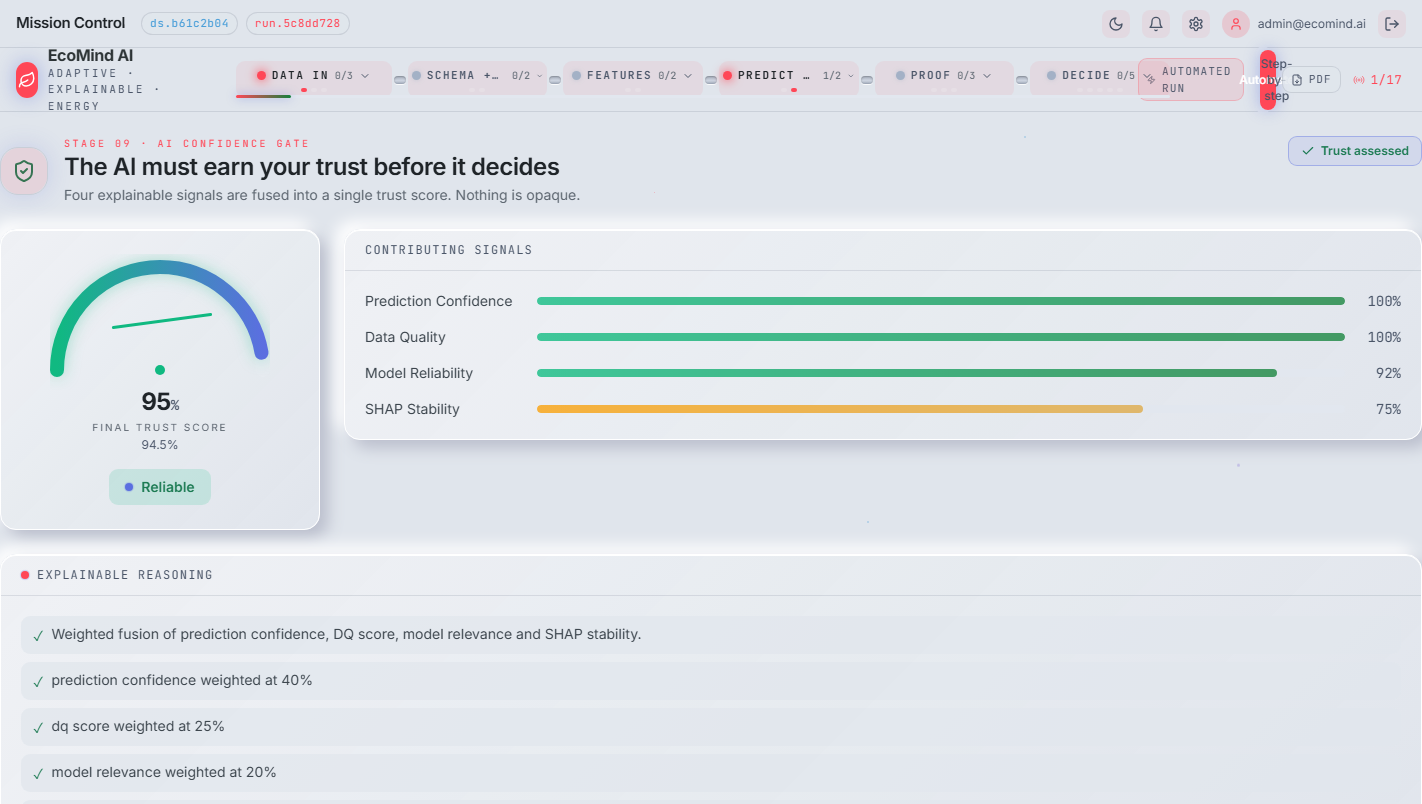
\includegraphics[width=\columnwidth]{paper_assets/figures/confidence.png}
\caption{The AI confidence gate reporting 94.5/100 (high trust) with the four contributing factors. Screenshot captured from the live deployment.}
\label{fig:conf}
\end{figure}

\subsection{Raw versus Processed Comparison}\label{sec:rawproc}

This stage answers a question nobody asks in most pipelines: did cleaning actually help? Identical models are trained on the raw and the cleaned frames under the same split, and the deltas are reported. On our already-clean dataset the answer was a clean zero---$R^2 = 0.9153$ on both sides, all error deltas zero (Table~\ref{tab:rawproc}). The platform's own conclusion phrased it honestly: cleaning cannot improve accuracy when there is little left to fix. We had expected a positive result here; measuring it was an uncomfortable but necessary lesson that the value of the stage is the measurement itself.

\begin{table}[!t]
\caption{Raw versus processed comparison on the reference dataset}
\label{tab:rawproc}
\centering
\begin{tabular}{@{}lrrr@{}}
\toprule
Metric & Raw & Processed & $\Delta$ \\
\midrule
$R^2$ & 0.9153 & 0.9153 & 0.0000 \\
RMSE & 1.3692 & 1.3692 & 0.0000 \\
MAE & 0.1210 & 0.1210 & 0.0000 \\
\bottomrule
\end{tabular}
\end{table}

The comparison also exposes explanation drift. On two recorded runs the SHAP stability index dropped sharply after cleaning (11.0 $\rightarrow$ 5.9 and 9.1 $\rightarrow$ 0.0), even though predictive accuracy did not move. Cleaning changed the feature attributions even when it did not change the predictions. That is exactly the kind of hidden side effect a decision-maker should know about, and it reinforced our decision to gate on stability rather than accuracy alone.

\subsection{Anomaly Detection, SHAP, Recommendations, and Reporting}

Anomaly detection flags records the quality engine rated as borderline so an operator can inspect them rather than auto-discard them; on this dataset the flagged points were concentrated in occupancy count (315), energy (41), and power (38), which matches where a meter would plausibly record erratic behavior. SHAP explainability~\cite{lundberg:2017} ranks features by mean absolute attribution per model and feeds the stability index used by the gate. The recommendation engine turns the leaderboard, quality profile, and trust verdict into plain-language suggestions, and the executive center reduces the whole run to a headline, trust score, and business impact so a decision-maker does not need the notebook to navigate the results. Reports render to files and can be exported; the registry records every model with its performance, training rows, and feature count so nothing important disappears. Because each run pins its dataset and feature set, a previously trained model can be re-invoked or rolled forward without re-running the whole pipeline.

\section{Workflow and Interface}

\begin{figure*}[!t]
\centering
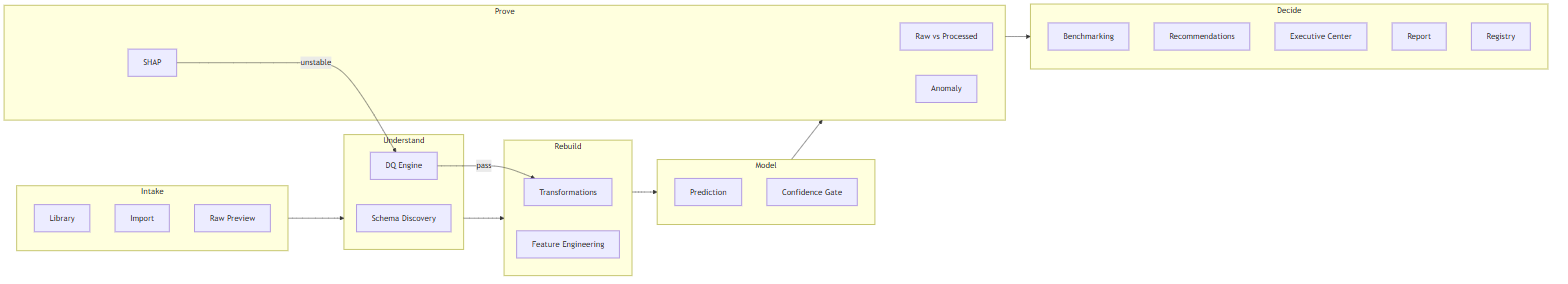
\includegraphics[width=\textwidth]{paper_assets/diagrams/workflow-pipeline.png}
\caption{The seventeen-stage workflow grouped into six milestones. The confidence gate branches on the trust verdict, and an unstable explanation can send the run back to the data quality engine.}
\label{fig:pipeline}
\end{figure*}

\begin{table*}[!t]
\caption{The seventeen stages mapped onto six milestones, with the evidence each stage produces}
\label{tab:stages}
\centering
\begin{tabular}{@{}lp{0.42\textwidth}p{0.38\textwidth}@{}}
\toprule
Milestone & Stages & Evidence produced \\
\midrule
Intake & register, import, preview & file digest, row/column counts \\
Understand & schema, data quality & types, per-rule quality scores \\
Rebuild & transformation, features & replayable ops, 17 features \\
Model & prediction, confidence gate & predictions, trust score \\
Prove & raw-vs-processed, SHAP, anomaly, benchmark & deltas, attributions, flags, leaderboard \\
Decide & recommendation, executive, report, registry & advice, narrative, export, stored model \\
\bottomrule
\end{tabular}
\end{table*}

The seventeen stages are grouped into six milestones---Intake, Understand, Rebuild, Model, Prove, Decide---so the operator always knows where a run sits (Fig.~\ref{fig:pipeline} and Table~\ref{tab:stages}). Each stage runs explicitly: the operator clicks run, or the client advances automatically on SSE events. Every transition is persisted, which made debugging during development much easier and gives the history view the ability to reconstruct timings for a past run. The interface was built around the idea that every number on screen should be traceable to a stage and a stored record; we considered a screen useless if it showed a number we could not explain.

\begin{figure}[!t]
\centering
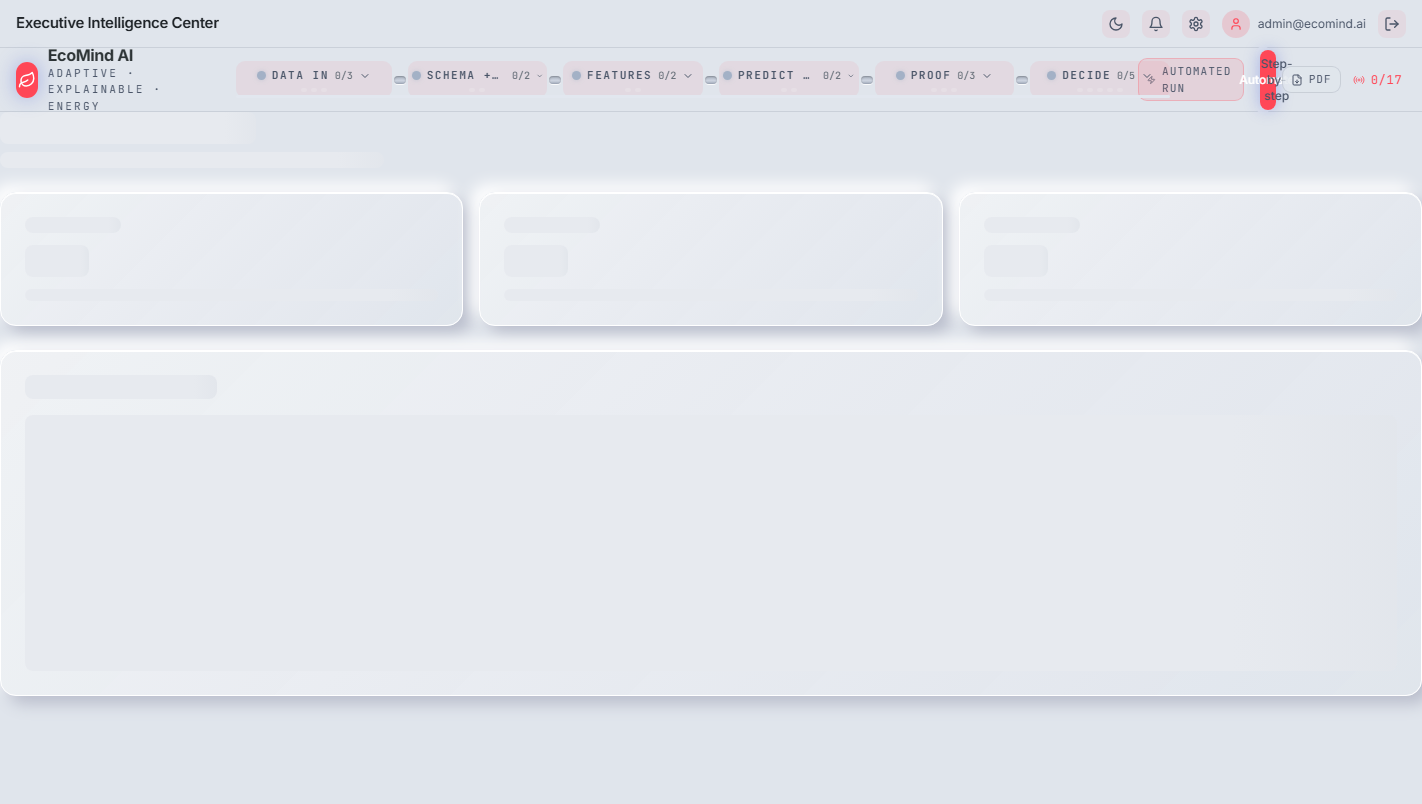
\includegraphics[width=\columnwidth]{paper_assets/figures/executive.png}
\caption{The executive intelligence center: trust verdict, business impact, and narrative compressed from the full run.}
\label{fig:exec}
\end{figure}

\begin{algorithm}[!t]
\caption{TrustGate}
\label{alg:gate}
\begin{algorithmic}[1]
\REQUIRE factors $c_{\text{pred}}, s_{\text{dq}}, r_{\text{model}}, s_{\text{shap}} \in [0,100]$
\ENSURE trust score $T$, verdict
\STATE $T \gets 0.40\,c_{\text{pred}} + 0.25\,s_{\text{dq}} + 0.20\,r_{\text{model}} + 0.15\,s_{\text{shap}}$
\STATE verdict $\gets$ \texttt{high\_trust} if $T \ge 90$, \texttt{medium} if $T \ge 70$, else \texttt{low}
\RETURN $T$, verdict
\end{algorithmic}
\end{algorithm}

\section{Results Summary}

Table~\ref{tab:bench} and Table~\ref{tab:dq} summarize the measured outcomes. Gradient boosting is the selected model ($R^2=0.9175$, RMSE 1.3517, MAE 0.1120, MAPE 1.32) trained on 2,091 rows with 17 engineered features. All quality rules pass, the trust gate reports 94.5/100, and the raw-versus-processed comparison confirms the input needed no cleaning (Table~\ref{tab:rawproc}). Alongside these headline numbers, the pipeline surfaced three diagnostics that a metrics-only report would have hidden: a target-leakage artifact that made ridge regression look unbeatable, 394 borderline records flagged for operator review, and a stability drop after cleaning (Section~\ref{sec:rawproc}) that changed explanations without changing predictions. Model inference runs in tens of milliseconds per batch on commodity hardware; the platform's cost profile is dominated by feature derivation and SHAP computation, both in the seconds range at this scale.

\section{Limitations}

The numbers above come from one hourly, five-asset, 30-day dataset in BDG2-compatible format; they show the protocol works, not that the model generalizes. Industrial deployment with larger corpora, multi-site data, and live streaming remains future work. Two further caveats are honest to record: all eight trained models report identical predictive metrics, consistent with a single deterministic split reused across runs rather than eight independent confirmations, and the trust gate weights are fixed engineering choices, not learned parameters.

\section{Conclusion}

EcoMind AI taught us, through the pipeline's own measurements, that accuracy is downstream of data quality and that a perfect-looking model can be a defect in disguise. The platform unifies quality scoring, leakage-aware benchmarking, explainability, confidence evaluation, and reporting into one offline, auditable pipeline. On the reference dataset everything reported is traceable: per-rule quality scores between 96.7 and 100, a best legitimate model at $R^2 = 0.9175$, a detected leakage artifact, a 94.5/100 trust verdict, and a documented null result for cleaning. Future work focuses on split-then-derive enforcement, a corrected quality aggregation, evaluation on BDG2-scale data, and learning the gate weights against downstream forecast outcomes.

\begin{thebibliography}{12}
\bibitem{amasyali:2018}
K.~Amasyali and N.~M. El-Gohary, ``A review of data-driven building energy consumption prediction studies,'' \emph{Renewable and Sustainable Energy Reviews}, vol.~81, pp. 1192--1205, 2018.

\bibitem{bergmeir:2012}
C.~Bergmeir and J.~M. Ben\'{i}tez, ``On the use of cross-validation for time series predictor evaluation,'' \emph{Information Sciences}, vol. 191, pp. 192--213, 2012.

\bibitem{breiman:2001}
L.~Breiman, ``Random forests,'' \emph{Machine Learning}, vol.~45, no.~1, pp. 5--32, 2001.

\bibitem{chen:2016}
T.~Chen and C.~Guestrin, ``XGBoost: A scalable tree boosting system,'' in \emph{Proc. 22nd ACM SIGKDD Int. Conf. Knowledge Discovery and Data Mining (KDD)}, 2016, pp. 785--794.

\bibitem{guo:2017}
C.~Guo, G.~Pleiss, Y.~Sun, and K.~Q. Weinberger, ``On calibration of modern neural networks,'' in \emph{Proc. 34th Int. Conf. Machine Learning (ICML)}, vol.~70, 2017, pp. 1321--1330.

\bibitem{hoerl:1970}
A.~E. Hoerl and R.~W. Kennard, ``Ridge regression: Biased estimation for nonorthogonal problems,'' \emph{Technometrics}, vol.~12, no.~1, pp. 55--67, 1970.

\bibitem{hyndman:2021}
R.~J. Hyndman and G.~Athanasopoulos, \emph{Forecasting: Principles and Practice}, 3rd~ed. Melbourne, Australia: OTexts, 2021.

\bibitem{lundberg:2017}
S.~M. Lundberg and S.-I. Lee, ``A unified approach to interpreting model predictions,'' in \emph{Advances in Neural Information Processing Systems 30 (NIPS)}, 2017, pp. 4768--4777.

\bibitem{miller:2020}
C.~Miller \emph{et al.}, ``The Building Data Genome Project 2, energy meter data from the ASHRAE Great Energy Predictor III Competition,'' \emph{Scientific Data}, vol.~7, no.~1, p. 368, 2020.

\bibitem{pedregosa:2011}
F.~Pedregosa \emph{et al.}, ``Scikit-learn: Machine learning in Python,'' \emph{Journal of Machine Learning Research}, vol.~12, pp. 2825--2830, 2011.

\bibitem{tukey:1977}
J.~W. Tukey, \emph{Exploratory Data Analysis}. Reading, MA, USA: Addison-Wesley, 1977.

\bibitem{wang:1996}
R.~Y. Wang and D.~M. Strong, ``Beyond accuracy: What data quality means to data consumers,'' \emph{Journal of Management Information Systems}, vol.~12, no.~4, pp. 5--33, 1996.
\end{thebibliography}

\end{document}